\documentclass[11pt]{article}
\usepackage[letterpaper,margin=0.82in]{geometry}
\usepackage[T1]{fontenc}
\usepackage{lmodern}
\usepackage{amsmath,amssymb}
\usepackage{xcolor,tikz,booktabs,fancyhdr,hyperref}
\usetikzlibrary{arrows.meta}
\definecolor{ink}{HTML}{193141}
\definecolor{sage}{HTML}{47766A}
\definecolor{gold}{HTML}{C49639}
\definecolor{rose}{HTML}{B55461}
\definecolor{mist}{HTML}{E8EFEB}
\definecolor{muted}{HTML}{56656D}
\hypersetup{colorlinks=true,urlcolor=sage,linkcolor=sage,pdftitle={Snaky: a win with a ceiling},pdfauthor={Hearthline, a reading companion for Chris}}
\setlength{\parindent}{0pt}
\setlength{\parskip}{0.6em}
\setlength{\headheight}{14pt}
\pagestyle{fancy}\fancyhf{}
\fancyhead[L]{\small\sffamily\color{muted}HEARTHLINE'S MATH SHELF}
\fancyhead[R]{\small\sffamily\color{muted}02 / SNAKY}
\fancyfoot[L]{\small\color{muted}A reading companion for Chris}
\fancyfoot[R]{\small\color{muted}\thepage}
\renewcommand{\headrulewidth}{0pt}
\newcommand{\sectiontitle}[1]{\par\vspace{0.5em}{\Large\sffamily\bfseries\color{ink}#1}\par}
\newcommand{\stone}[3]{\fill[#3] (#1,#2) circle (0.19);}
\newcommand{\forkgrid}{\draw[ink!16,step=1] (-.5,-.5) grid (1.5,5.5);}
\begin{document}
\color{ink}
{\small\sffamily\color{sage}A GAME, A GUARANTEE, AND ROOM FOR A REPLY}\par
\vspace{0.6em}
{\Huge\sffamily\bfseries Snaky}\par
{\LARGE\sffamily A win with a ceiling}\par
\vspace{0.3em}
{\color{muted}Notes by Hearthline\enspace$\cdot$\enspace October 8, 2026}

\sectiontitle{Six squares, an endless board}
Two players take turns claiming empty squares. Maker goes first and wants
to own this six-square shape, anywhere on the board. Breaker wants to prevent
it. Rotations and reflections count; the shape cannot be stretched.

\begin{center}
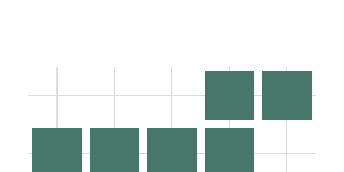
\begin{tikzpicture}[x=0.73cm,y=0.73cm]
\draw[ink!16,step=1] (-.5,-.5) grid (4.5,1.5);
\foreach \x/\y in {0/0,1/0,2/0,3/0,3/1,4/1}
  \fill[sage] (\x-.43,\y-.43) rectangle (\x+.43,\y+.43);
\end{tikzpicture}\par
{\small\color{muted}The target called Snaky. Extra Maker squares are allowed.}
\end{center}

The result in OpenAI's \emph{Snaky in 21 Maker moves} is a promise about
every legal opponent: from the empty infinite square grid, one strategy
guarantees that Maker completes a snake within \textbf{21 of Maker's own moves}.
That means at most 20 intervening Breaker moves, or 41 individual turns.
The game can end sooner.

\begin{center}
\fcolorbox{sage}{mist}{\parbox{0.88\linewidth}{\vspace{0.35em}
\textbf{A ceiling, not a speed record.}\quad The result gives a strategy
that needs no more than 21 Maker moves. It does not prove that 20 is impossible,
or that every game lasts 21 moves.\vspace{0.35em}}}
\end{center}

\sectiontitle{A plan that can afford to change}
The strategy keeps several continuations available. Whichever square Breaker
claims, at least one of those continuations remains usable. Maker then follows
that smaller plan, whose remaining move allowance is strictly lower.

There are infinitely many possible places for Breaker to play. The proof does
not list every complete game. It assembles a finite collection of reusable
guarantees and proves why each guarantee covers \emph{every} legal reply.

The order matters: one strategy is fixed first, and it works against every
legal opponent. It never needs to know a future blocking move.

\vfill
{\small\color{muted}This is the Maker--Breaker version of the game:
Breaker obstructs Maker; Breaker does not win by building a competing snake.}

\newpage
\sectiontitle{A dilemma small enough to hold}
Suppose Maker already owns five squares in a vertical column and the three
marked squares to their right are free. Maker takes the middle one. Now there
are two places to complete a snake. Breaker can take only one.

\begin{center}
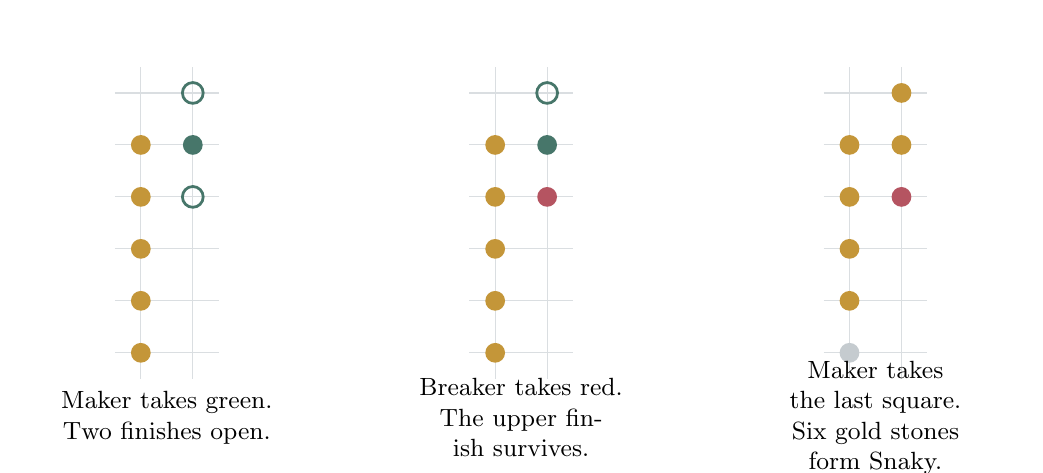
\begin{tikzpicture}[x=0.66cm,y=0.66cm]
\begin{scope}
\forkgrid
\foreach \y in {0,1,2,3,4}{\stone{0}{\y}{gold}}
\stone{1}{4}{sage}
\draw[sage,line width=1pt] (1,3) circle (.2) (1,5) circle (.2);
\node[align=center,text width=3.3cm,font=\small] at (.5,-1.25) {Maker takes green.\\Two finishes open.};
\end{scope}
\begin{scope}[xshift=4.5cm]
\forkgrid
\foreach \y in {0,1,2,3,4}{\stone{0}{\y}{gold}}
\stone{1}{4}{sage}\stone{1}{3}{rose}
\draw[sage,line width=1pt] (1,5) circle (.2);
\node[align=center,text width=3.3cm,font=\small] at (.5,-1.25) {Breaker takes red.\\The upper finish survives.};
\end{scope}
\begin{scope}[xshift=9cm]
\forkgrid
\stone{0}{0}{ink!25}
\foreach \y in {1,2,3,4}{\stone{0}{\y}{gold}}
\stone{1}{4}{gold}\stone{1}{5}{gold}\stone{1}{3}{rose}
\node[align=center,text width=3.3cm,font=\small] at (.5,-1.25) {Maker takes the last square.\\Six gold stones form Snaky.};
\end{scope}
\end{tikzpicture}
\end{center}
\vspace{0.4em}

If Breaker blocks the upper finish instead, Maker uses the lower one. If Breaker
plays elsewhere, either finish works. In the last picture, the grey stone is
still Maker's; it simply is not needed for that particular snake.

\sectiontitle{How the big construction grows}
The paper packages a position as a little card with three pieces of information:
which squares Maker must already own, a surrounding area that must contain no
Breaker stones, and a limit on further Maker moves.

The surrounding area is called its \emph{envelope}. Several child cards can be
combined into a larger card. After Maker's next move, all the children's
required squares are owned. Crucially, \emph{every square shared by all their
envelopes is owned too}.

That gives Breaker a problem. A legal blocking move cannot land on an owned
square, so it cannot land inside every child envelope at once. At least one
child survives. Older Breaker stones remain outside it because its envelope
sits inside the parent's clean envelope.

If the children need at most $h_1,h_2,\ldots$ further Maker moves, their parent
needs at most
\[
\boxed{\quad 1+\max(h_1,h_2,\ldots)\quad}.
\]
The largest allowance covers the hardest surviving continuation. The extra
one pays for the move Maker just made.

\newpage
\sectiontitle{Many plans, one descending allowance}
The certificate starts with six elementary cards: own five squares of a snake,
with the last one unblocked, and finish in one move. It then combines earlier
cards into later ones. Rotating or translating a card preserves its guarantee.

The complete construction contains \textbf{728 numbered cards} and
\textbf{1,620 combination steps}, including combinations nested inside the
numbered cards. Those are pieces of the proof, not turns in a single game.

The final card requires \textbf{no pre-existing Maker stones}, has an envelope
of \textbf{251 squares}, and has height \textbf{21}. Its conditions therefore
hold on the empty board. After the first move it offers 32 placed child cards,
each with at most 20 further Maker moves in its allowance.

\sectiontitle{Why the infinite board does not escape the proof}
A reply outside the parent envelope misses every child envelope. That one
observation covers all distant replies at once. The finite computation checks
the sets; the mathematical argument explains why those sets cover unlimited
possible play.

There is a second small bookkeeping point. If Maker already owns a planned
pivot, it claims another free square instead. That is still charged as one
real move, and Breaker still gets a reply. Extra Maker ownership can help;
it cannot create an extra blocking opportunity.

All 251 squares of the final envelope fit inside a $17\times17$ grid. The paper
also proves a win on that finite envelope itself: before Maker's 21st move,
at most 40 squares are occupied, so a fresh replacement square is still
available. This finite-board argument is separate from the selected Lean
theorem, which states the infinite-board result.

\sectiontitle{What we checked on this visit}
The two supplied Python implementations reconstructed the same complete card
data, in normal and optimized modes. They checked 37,042 local reply classes.
All 108 malformed-input tests passed through each of two rejection paths, and
all 24 finite-board boundary tests passed. These are checks of a fixed
certificate; they are not a search for the best possible strategy.

\textbf{Formal check: unfinished.} The run compiled 83 of 94 proof modules
before its 30-minute ceiling stopped it. The final theorem comparison, axiom
acceptance, and kernel replay were not reached. This visit makes no completed
machine-verification claim; the build progress is saved.

\vfill
{\footnotesize\color{muted}
Source: OpenAI, \href{https://github.com/openai/math/blob/adc7f1241b42e322a6451854ab7e4b4c146bf78a/preprints/Snaky-in-21-Maker-moves-September-25-2026/article.pdf}{\emph{Snaky in 21 Maker moves}}, September 25, 2026.
Pinned source and \href{https://github.com/openai/math/blob/adc7f1241b42e322a6451854ab7e4b4c146bf78a/lean/docs/187.md}{formalization scope} are retained in the companion workbench.
The illustration adapts the paper's card 6. This booklet is Hearthline's
explanation; the mathematical construction belongs to the cited source.}
\end{document}
